\subsection{Physarum Polycephalum}
\label{sub:PhysarumArte}
    %Parrafo 1
    En esta secci\'on nos concentraremos principamente en los diferentes modelos que se han propuesto para modelar el 
        Physarum Polycephalum, as\'i como en las aplicaciones que se han desarrollado a partir de estos modelos.
        Principalmente son 5 los modelos que se han propuesto para modelar el Physarum Polycephalum, los cuales son:
        el modelado de Adamatzky, el modelado de Olvera, el modelado de Mar\'in, el modelado de Jones y el modelado de
        Gunji. A continuaci\'on, se describir\'an brevemente cada uno de estos modelos.
    \clearpage
\subsubsection{Modelado de Adamatzky}

    El modelo de \textit{Physarum polycephalum} de Andrew Adamatzky destaca sus capacidades computacionales. 
        Manipulando \textit{Physarum} con alimentos y repelentes, demuestra la creaci\'on de puertas l\'ogicas y 
        la resoluci\'on de problemas de optimizaci\'on como el camino m\'as corto y el problema del agente viajero \cite{Adamatzky2010}.
        En la Figura \ref{fig:puertas_logicas} se muestra un ejemplo de puertas l\'ogicas creadas por \textit{Physarum}.
    \vskip 0.5cm
    % Imagen 1: Ejemplo de puertas l\'ogicas creadas por Physarum
    \begin{figure}[h]
        \centering
        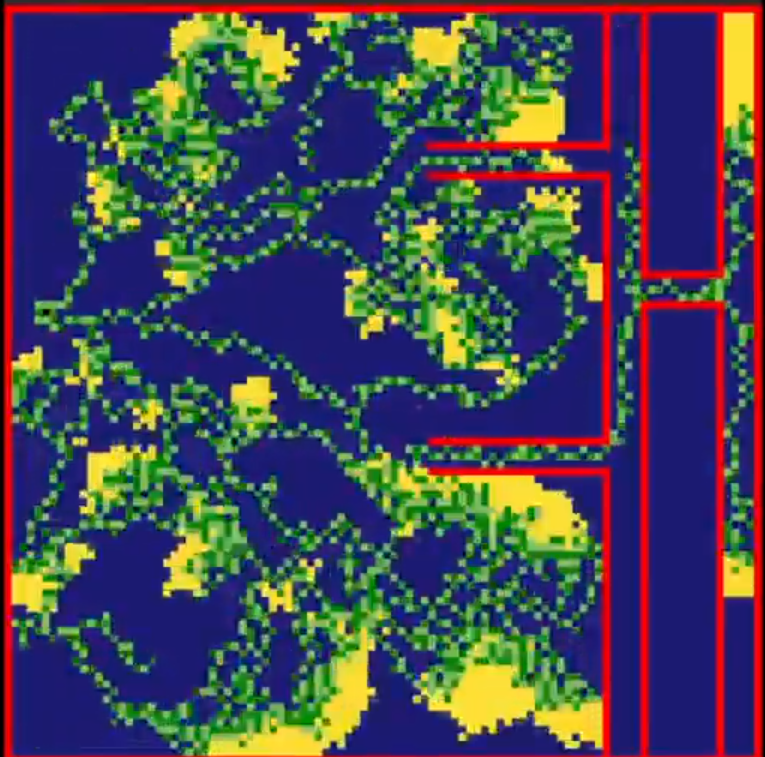
\includegraphics[width=0.5\textwidth]{./images/estado_del_arte/physarum/CompuertasLogicas.png}
        \caption{Ejemplo de puertas l\'ogicas (OR) creadas por \textit{Physarum}.}
        \label{fig:puertas_logicas}
    \end{figure}
    \vskip 0.5cm
    Adamatzky profundiza en la red protoplasm\'atica de \textit{Physarum}, compar\'andola con sistemas humanos, y 
        muestra propiedades memristivas similares a los memristores electr\'onicos \cite{Adamatzky2010}. Su investigaci\'on 
        tambi\'en explora la din\'amica no lineal y la formaci\'on de patrones complejos, significativos para la computaci\'on 
        no convencional \cite{Adamatzky2010}.
    \vskip 0.5cm
    El modelo utiliza part\'iculas de enjambre en un entorno bidimensional (2D) para simular el movimiento ameboide de 
        \textit{Physarum}. Estas part\'iculas tienen etapas sensitiva y motora, interactuando con un quimioatrayente 
        y generando patrones complejos. Adem\'as, se considera la resistencia al movimiento y la influencia de est\'imulos 
        externos como quimioatrayentes y luz, controlando el comportamiento del colectivo.
    \vskip 0.5cm
    Una caracter\'istica destacada es la capacidad del colectivo para cambiar y recuperar su forma, navegar obst\'aculos 
        y dividirse en fragmentos independientes que pueden fusionarse nuevamente, lo cual es deseable en aplicaciones 
        rob\'oticas \cite{Adamatzky2010}. La Figura \ref{fig:adaptacion_obstaculos} ilustra c\'omo el colectivo de 
        \textit{Physarum} se adapta a obst\'aculos.
    \vskip 0.5cm
    % Imagen 2: Colectivo de Physarum adapt\'andose a obst\'aculos
    \begin{figure}[h]
        \centering
        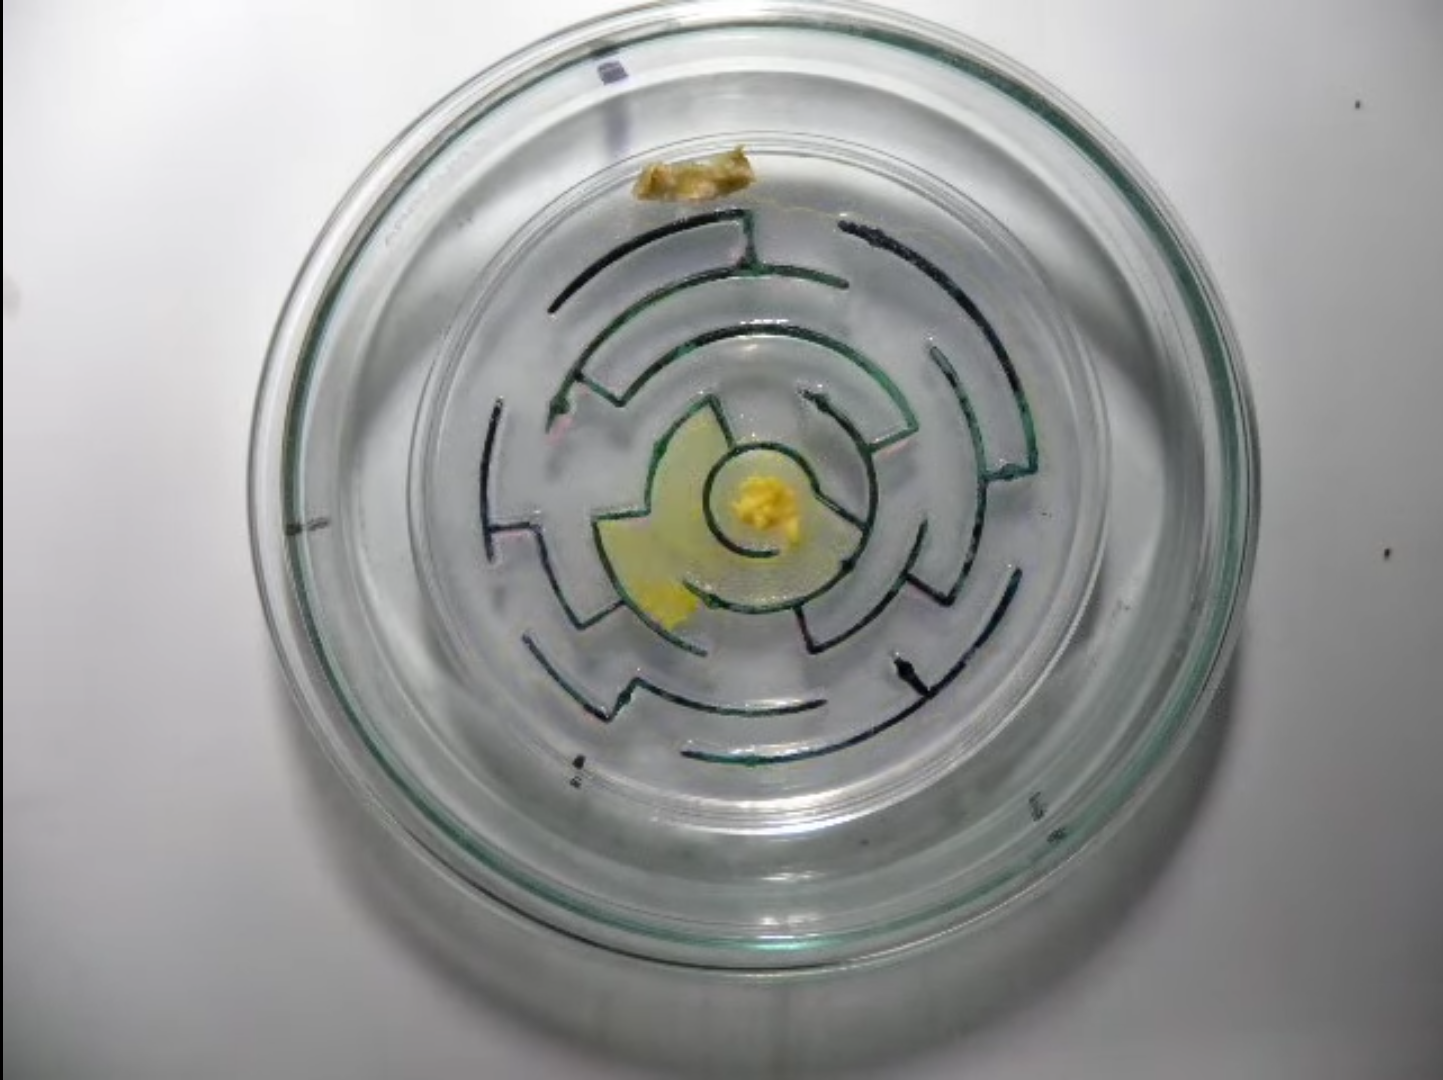
\includegraphics[width=0.5\textwidth]{./images/estado_del_arte/physarum/laberinto.png}
        \caption{Colectivo de \textit{Physarum} adapt\'andose a obst\'aculos. \cite{Adamatzky_2012}}
        \label{fig:adaptacion_obstaculos}
    \end{figure}
    \vskip 0.5cm
    Para m\'as detalles, ver '\textit{Emergence of self-organized amoeboid movement in a multi-
    agent approximation of physarum polycephalum}' \cite{jones2012}.

    \subsubsection{Modelado Guillermo Olvera} % (fold)
\label{ssub:ModeladoGuillermoOlvera}
    El modelo utiliza aut\'omatas celulares con la vecindad de Moore para simular la propagaci\'on y b\'usqueda de rutas del organismo 
        \textit{Physarum Polycephalum}. Este modelo funciona en una cuadr\'icula bidimensional donde cada c\'elula puede asumir 
        uno de varios estados: campo libre, nutriente no encontrado, repelente, punto inicial, gel en contracci\'on, 
        gel en compuesto, nutriente hallado, expansi\'on del \textit{Physarum} y gel sin compuesto.
    \vskip 0.5cm
    El algoritmo est\'a implementado en Python, lo cual introduce ciertas limitaciones en t\'erminos de 
        velocidad y escalabilidad. Debido a la naturaleza interpretada de Python, el modelo es lento 
        y poco escalable cuando se incrementa el n\'umero total de c\'elulas e hilos utilizados.
    \vskip 0.5cm
    El proceso comienza con la designaci\'on de una c\'elula inicial que representa el punto de inicio del \textit{Physarum}. 
        Las reglas de transici\'on determinan c\'omo cambian los estados de las c\'elulas en funci\'on de sus vecinos. Por ejemplo, 
        una c\'elula de campo libre se convierte en una c\'elula de expansi\'on del \textit{Physarum} si est\'a adyacente a una 
        c\'elula en estado de punto inicial, gel en contracci\'on o nutriente hallado. Las c\'elulas de expansi\'on del \textit{Physarum} 
        se propagan por la cuadr\'icula, y al encontrarse con nutrientes, estas c\'elulas cambian su estado a nutriente hallado, 
        lo que refuerza la ruta. En la Figura \ref{fig:initial_state} se muestra la configuraci\'on inicial del \textit{Physarum} en la cuadr\'icula.
    \vskip 0.5cm
    \begin{figure}[h]
        \centering
        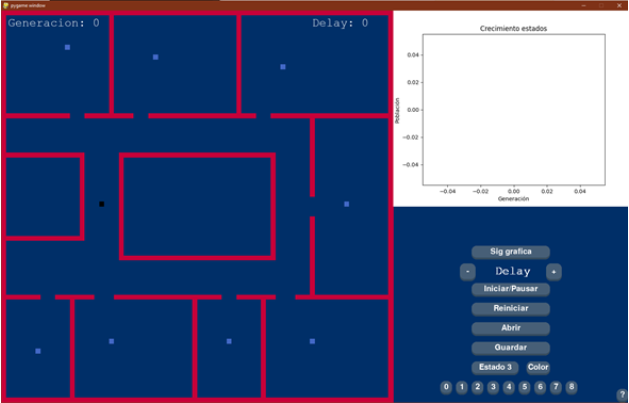
\includegraphics[width=0.5\textwidth]{./images/estado_del_arte/physarum/estadoInicialOlvera.png}
        \caption{Configuraci\'on inicial del \textit{Physarum} en la cuadr\'icula. \cite{Olvera2023}}
        \label{fig:initial_state}
    \end{figure}
    \vskip 0.5cm
    A medida que el \textit{Physarum} se expande, se generan rutas que conectan las fuentes de nutrientes, 
        adapt\'andose din\'amicamente a la presencia de obst\'aculos y asegurando la conectividad en el entorno. Aunque el 
        algoritmo garantiza la formaci\'on de al menos una ruta viable, la trayectoria del \textit{Physarum} no es 
        realmente aleatoria, ya que sigue patrones determinados por las reglas de transici\'on. Estas reglas, sin embargo,
        no siempre son claras ni consistentes. En la Figura \ref{fig:expansion} se muestra la expansi\'on del \textit{Physarum} y la formaci\'on de rutas.
    \vskip 0.5cm
    \begin{figure}[h]
        \centering
        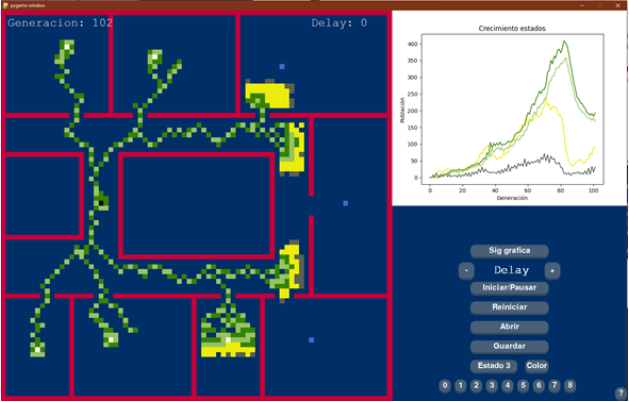
\includegraphics[width=0.5\textwidth]{./images/estado_del_arte/physarum/expansionOlvera.png}
        \caption{Expansi\'on del \textit{Physarum} y formaci\'on de rutas. \cite{Olvera2023}}
        \label{fig:expansion}
    \end{figure}
    \vskip 0.5cm
    Las reglas de transici\'on se definen para cada estado de la c\'elula, 
        asegurando que el \textit{Physarum} pueda encontrar y seguir rutas hacia los nutrientes, 
        adapt\'andose en tiempo real a cambios en el entorno. Sin embargo, estas reglas no 
        siempre son claras ni est\'an bien documentadas en la referencia \cite{Olvera2023}.

    % subsubsection Modelado Guillermo Olvera (end)
    \subsubsection{Modelado de Yair Marin} % (fold)
\label{ssub:ModeladodeYairMarin}
    El algoritmo utilizado para modelar el comportamiento del \textit{Physarum Polycephalum} 
        en el documento se basa en aut\'omatas celulares y se define por un conjunto de estados 
        y reglas de transici\'on espec\'ificas. Los estados incluyen campo libre, nutriente no 
        encontrado, repelente, punto inicial, gel en contracci\'on, gel con compuesto, 
        nutriente hallado, expansi\'on del \textit{Physarum} y gel sin compuesto. 
        Estos estados evolucionan de acuerdo con la vecindad de von Neumann, que 
        considera las c\'elulas adyacentes en las direcciones norte, sur, este y oeste.
    \vskip 0.5cm
    Las reglas de transici\'on determinan c\'omo cambia el estado de cada c\'elula en funci\'on de 
        sus vecinos. Por ejemplo, una c\'elula en estado de campo libre (q0) puede pasar al 
        estado de expansi\'on del \textit{Physarum} (q7) si est\'a adyacente a un punto inicial 
        (q3), gel en contracci\'on (q4) o nutriente hallado (q6). Del mismo modo, una c\'elula en 
        estado de nutriente no encontrado (q1) cambia a estado de nutriente hallado (q6) si 
        est\'a cerca de un gel con compuesto (q5) o otro nutriente hallado (q6). Estas reglas 
        permiten que el modelo emule el comportamiento del \textit{Physarum} en la b\'usqueda y 
        exploraci\'on de su entorno, formando redes eficientes para el transporte de nutrientes 
        y adapt\'andose a cambios en el entorno \cite{MarinAlavez2018}.
    \vskip 0.5cm
    En la Figura \ref{fig:algorithm_running}, se muestra una ejecuci\'on del algoritmo, demostrando 
        c\'omo el \textit{Physarum} se expande y encuentra nutrientes en un entorno simulado.

    % Imagen del algoritmo corriendo
    \begin{figure}[h]
        \centering
        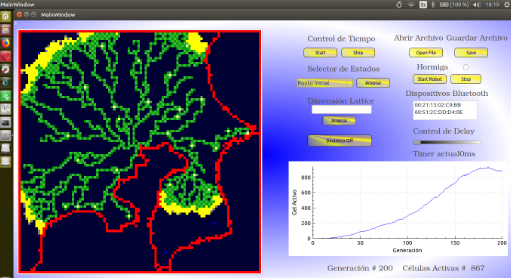
\includegraphics[width=0.7\textwidth]{./images/estado_del_arte/physarum/yahirPrograma.png}
        \caption{Ejecuci\'on del algoritmo de \textit{Physarum Polycephalum} encontrando nutrientes. \cite{MarinAlavez2018}}
        \label{fig:algorithm_running}
    \end{figure}
% subsubsection Modelado de Yahir Marin (end)
    \clearpage
\subsubsection{Modelado de Jeff Jones} % (fold)
\label{ssub:jones}
    El algoritmo propuesto en 'From Pattern Formation to Material Computation: Multi-agent Modelling of Physarum Polycephalum' 
        \cite{Jones2015} aprovecha el comportamiento natural de \textit{Physarum polycephalum} para resolver problemas 
        computacionales mediante un marco de sistema multiagente (MAS). El n\'ucleo del algoritmo involucra un gran n\'umero de 
        agentes simples que imitan el comportamiento del plasmodio de \textit{Physarum}. Cada agente opera basado en reglas 
        locales, movi\'endose e interactuando dentro de un entorno virtual que simula el espacio f\'isico donde reside el moho del limo.
    \vskip 0.5cm
    Los agentes se mueven hacia las fuentes de nutrientes siguiendo gradientes qu\'imicos, representando las se\~nales atrayentes 
        utilizadas por \textit{Physarum}. Dejan rastros similares a feromonas que refuerzan los caminos exitosos, de manera similar 
        a c\'omo \textit{Physarum} fortalece sus tubos protoplasm\'aticos. Este mecanismo de retroalimentaci\'on de feromonas permite 
        que los agentes se adapten din\'amicamente a los cambios en el entorno, optimicen caminos y encuentren soluciones a 
        problemas como el camino m\'as corto o la resoluci\'on de laberintos. El comportamiento colectivo de estos agentes 
        simples conduce a la emergencia de redes complejas y eficientes que pueden ser utilizadas para tareas de computaci\'on no convencional.
    \vskip 0.5cm
    La fortaleza del algoritmo radica en su capacidad de autoorganizaci\'on y adaptaci\'on sin control central. 
        Demuestra capacidades robustas de resoluci\'on de problemas incluso en entornos din\'amicos e inciertos. Al aprovechar 
        los principios de autoorganizaci\'on e interacci\'on local, el algoritmo ofrece un enfoque novedoso para la computaci\'on 
        distribuida y la optimizaci\'on, inspirado en el comportamiento natural de \textit{Physarum polycephalum}.
    \vskip 0.5cm
    % Imagen 1: Representaci\'on del agente de acuerdo con el modelo de Jeff Jones
    En la Figura \ref{fig:pseudocodigo} se muestra una representaci\'on del agente de acuerdo con el modelo de Jeff Jones.
    % Imagen del pseudoc\'odigo del algoritmo
    \begin{figure}[h]
        \centering
        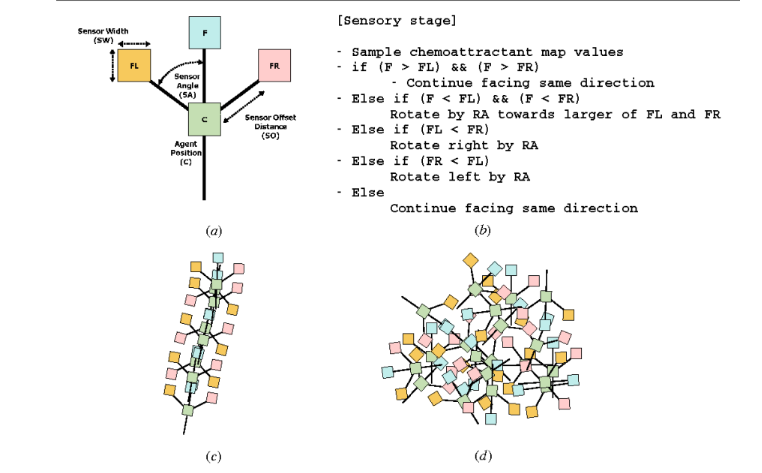
\includegraphics[width=0.7\textwidth]{./images/estado_del_arte/physarum/pseudoJones.png}
        \caption{Representaci\'on del agente de acuerdo con el modelo de Jeff Jones. \cite{Jones2015}}
        \label{fig:pseudocodigo}
    \end{figure}
\clearpage
    \subsubsection{Modelado de Gunji} % (fold)
\label{ssub:Modelado de Gunji}

    El modelo de c\'elula m\'inima inspirado en el comportamiento del moho del limo \textit{Physarum polycephalum} 
        simula la capacidad de la c\'elula para moverse y resolver problemas complejos como laberintos y 
        configuraciones de \'arboles generadores a trav\'es de mecanismos simples pero efectivos. La c\'elula 
        est\'a representada en una rejilla plana, donde cada sitio puede estar en uno de varios estados: 
        externo (0), interno (1), l\'imite (2) o estado final (-1). El modelo presenta dos fases principales: 
        desarrollo y b\'usqueda de alimento. Durante la fase de desarrollo, la c\'elula crece desde una semilla 
        inicial hasta formar una agregaci\'on estructurada, mientras que en la fase de b\'usqueda de alimento, 
        modifica activamente su forma y se mueve 'comiendo' sitios externos, causando flujo citoplasm\'atico 
        y reorganizaci\'on de los l\'imites.
    \vskip 0.5cm
    Un aspecto clave del modelo es el proceso de 'comer 0', donde un sitio en estado 0 (externo) invade la c\'elula, 
        convirti\'endose en una 'burbuja' que es transportada dentro de la c\'elula sin cruzar su propio camino 
        (flujo memorizado). Este proceso conduce a la formaci\'on y eliminaci\'on de tent\'aculos, creaci\'on de redes 
        adaptativas y optimizaci\'on de caminos para resolver problemas como laberintos y configuraciones de 
        \'arboles generadores. La interacci\'on entre el flujo citoplasm\'atico local y la forma global de la c\'elula, 
        impulsada por la alternancia entre endurecimiento y ablandamiento citoplasm\'atico, permite que la c\'elula 
        se adapte din\'amicamente y mantenga su estructura, exhibiendo comportamientos similares a la resoluci\'on 
        inteligente de problemas observada en \textit{Physarum polycephalum} \cite{gunji2008}.
    \vskip 0.5cm
    En la Figura \ref{fig:cell_algorithm}, se muestra c\'omo se aplica el algoritmo para resolver un laberinto. 
        Este ejemplo ilustra la capacidad del modelo para adaptarse y optimizar caminos en tiempo real.
    \vskip 0.5cm
    % Imagen del algoritmo siendo usado
    \begin{figure}[h]
        \centering
        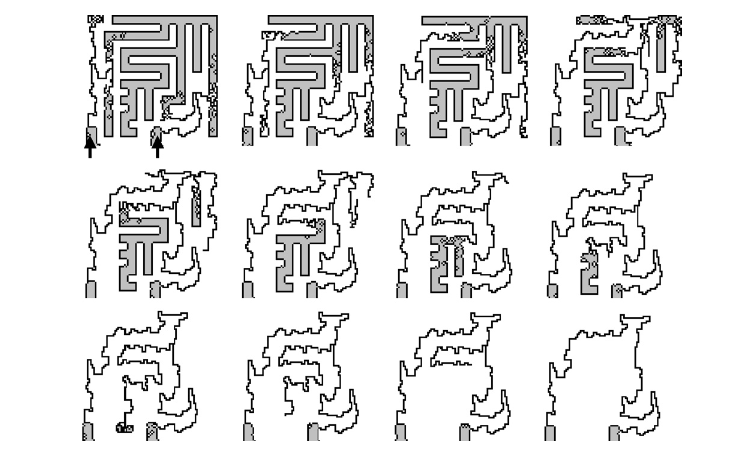
\includegraphics[width=0.7\textwidth]{./images/estado_del_arte/physarum/laberintoGunji.png}
        \caption{Aplicaci\'on del algoritmo para resolver un laberinto utilizando el modelo de \textit{Physarum polycephalum}. \cite{gunji2008}}
        \label{fig:cell_algorithm}
    \end{figure}
    \vskip 0.5cm
    Las reglas del modelo se describen en la Figura \ref{fig:cell_rules}, mostrando los diferentes 
        estados de los sitios y c\'omo interact\'uan durante las fases de desarrollo y b\'usqueda de alimento.
    \vskip 0.5cm
    % Imagen de las reglas del modelo
    \begin{figure}[h]
        \centering
        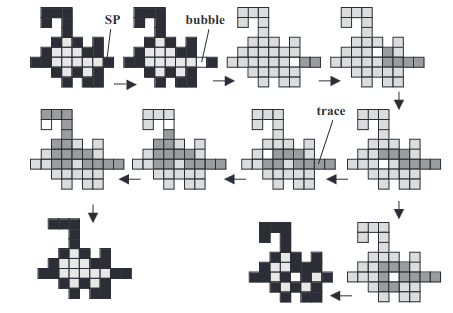
\includegraphics[width=0.7\textwidth]{./images/estado_del_arte/physarum/rGunji.png}
        \caption{Reglas del modelo de c\'elula m\'inima, mostrando los estados de los sitios y las interacciones. \cite{gunji2008}}
        \label{fig:cell_rules}
    \end{figure}
